\documentclass[conference]{IEEEtran}
\IEEEoverridecommandlockouts

% ================= PACKAGES =================
\usepackage{cite}
\usepackage{amsmath,amssymb,amsfonts}
\usepackage{graphicx}
\usepackage[utf8]{inputenc}
\usepackage{textgreek}
\usepackage{textcomp}
\usepackage{xcolor}
\usepackage{caption}
\usepackage{subcaption}
\usepackage{booktabs}
\usepackage{gensymb}
\usepackage{multirow}
\usepackage{array}
\usepackage{float}
\usepackage{siunitx}
\usepackage{epstopdf}


\def\BibTeX{{\rm B\kern-.05em{\sc i\kern-.025em b}\kern-.08em
    T\kern-.1667em\lower.7ex\hbox{E}\kern-.125emX}}

\begin{document}

\title{Analysis and Design of a Telescopic Operational Amplifier in 180 nm CMOS Technology}

\author{
\IEEEauthorblockN{Siddhant Shah (B23334)\textsuperscript{*}, 
                  Aman (T25121)\textsuperscript{†}, 
                  Omkar Sharan (T25132)\textsuperscript{‡}}
\IEEEauthorblockA{\textsuperscript{*}b23334@students.iitmandi.ac.in \\
                  \textsuperscript{†}t25121@students.iitmandi.ac.in \\
                  \textsuperscript{‡}t25132@students.iitmandi.ac.in}
}

\maketitle

% ================= ABSTRACT =================
\begin{abstract}
\noindent
This paper presents the systematic design and analysis of a telescopic operational amplifier implemented in SCL 180 nm CMOS technology. The design targets a closed-loop gain of 50 dB and unity-gain bandwidth (UGBW) of 100 MHz while operating at a supply voltage of 1.8 V. The telescopic architecture employs cascoded differential pairs with active loads to achieve high gain and moderate power consumption. Through careful transistor sizing and bias optimization, the implemented design achieved a small-signal DC gain of 63 dB, UGBW of 100.78 MHz, phase margin of 68°, PSRR of 11.18 dB, CMRR of 58 dB, and input-referred noise of approximately 15 nV/$\sqrt{\text{Hz}}$. The design methodology, transistor sizing, simulation results, and performance analysis are presented in detail.
\end{abstract}

\begin{IEEEkeywords}
Telescopic amplifier, operational amplifier, CMOS, gain, unity-gain bandwidth, phase margin, noise, PSRR, CMRR, 180 nm technology, analog IC design
\end{IEEEkeywords}

% ================= INTRODUCTION =================
\section{Introduction}
\noindent
Operational amplifiers are fundamental building blocks in analog and mixed-signal integrated circuits, finding widespread applications in signal processing, data converters, filters, and sensor interfaces \cite{razavi, gray}. Among various op-amp topologies, the telescopic architecture offers an attractive balance between high DC gain, moderate bandwidth, and reasonable power consumption \cite{johns}.

\noindent
The telescopic operational amplifier achieves high open-loop gain through vertical stacking of cascoded transistors, which significantly increases the output impedance while maintaining a compact circuit structure \cite{baker}. Unlike folded-cascode topologies, telescopic amplifiers consume less power as all transistors share the same bias current path. However, this comes at the cost of reduced output voltage swing due to the stacked transistor configuration \cite{razavi}.

\noindent
This work focuses on designing a two-stage telescopic op-amp for general-purpose analog applications where high gain and moderate bandwidth are essential. The design targets include:
\begin{itemize}
    \item DC gain of at least 50 dB
    \item Unity-gain bandwidth of 100 MHz
    \item Low input-referred noise
    \item Stable operation with adequate phase margin
    \item Good common-mode and power supply rejection
\end{itemize}

\noindent
The choice of 180 nm CMOS technology provides a mature process with well-characterized device models, making it suitable for educational purposes and prototyping. The 1.8 V supply voltage is standard for this technology node.

\noindent
This paper is organized as follows: Section II presents the design specifications and process parameters. Section III describes the circuit topology and design methodology including transistor sizing. Section IV presents the simulation results and performance verification. Section V provides discussion and analysis. Section VI concludes the work.

% ================= DESIGN SPECIFICATIONS =================
\section{Design Specifications}
\noindent
The target specifications for the telescopic operational amplifier design are summarized in Table~\ref{tab:specs}. These specifications are derived from typical requirements for medium-performance analog applications such as active filters and moderate-resolution data converters.

\begin{table}[H]
    \centering
    \caption{Design Specifications and Targets}
    \label{tab:specs}
    \begin{tabular}{@{}lc@{}}
        \toprule
        \textbf{Parameter} & \textbf{Target Value} \\
        \midrule
        Technology & SCL 180 nm CMOS \\
        Supply Voltage ($V_{DD}$) & 1.8 V \\
        DC Gain (Open-loop) & $\geq$ 50 dB \\
        Unity-Gain Bandwidth & 100 MHz \\
        Phase Margin & $\geq$ 60\degree \\
        Load Capacitance ($C_L$) & 1 pF \\
        CMRR & High \\
        \bottomrule
    \end{tabular}
\end{table}

\subsection{Process Parameters}
\noindent
The design utilizes the SCL 180 nm CMOS process technology. The key process parameters are listed in Table~\ref{tab:process}, which are essential for transistor sizing and performance estimation.

\begin{table}[H]
    \centering
    \caption{SCL 180 nm CMOS Process Parameters}
    \label{tab:process}
    \begin{tabular}{@{}lcc@{}}
        \toprule
        \textbf{Parameter} & \textbf{NMOS} & \textbf{PMOS} \\
        \midrule
        Mobility ($\mu$) & 300 cm$^2$/Vs & 70 cm$^2$/Vs \\
        Oxide Capacitance ($C_{ox}$) & \multicolumn{2}{c}{8.78 fF/$\mu$m$^2$} \\
        $\mu C_{ox}$ & 263 $\mu$A/V$^2$ & 62 $\mu$A/V$^2$ \\
        Threshold Voltage ($V_{TH}$) & 0.48 V & -0.40 V \\
        Channel-length modulation ($\lambda$) & 0.48 V$^{-1}$ & 0.328 V$^{-1}$ \\
        Oxide Thickness ($T_{ox}$) & \multicolumn{2}{c}{4 nm} \\
        Minimum Length ($L_{min}$) & \multicolumn{2}{c}{180 nm} \\
        \bottomrule
    \end{tabular}
\end{table}

% ================= DESIGN METHODOLOGY =================
\section{Design Methodology}

\subsection{Circuit Topology and Operation}
\noindent
\noindent
The complete schematic of the designed telescopic operational amplifier is shown in Fig.~\ref{fig:ckt}. The circuit implements a two-stage architecture with Miller compensation for stability.

\begin{figure*}[t]
    \centering
    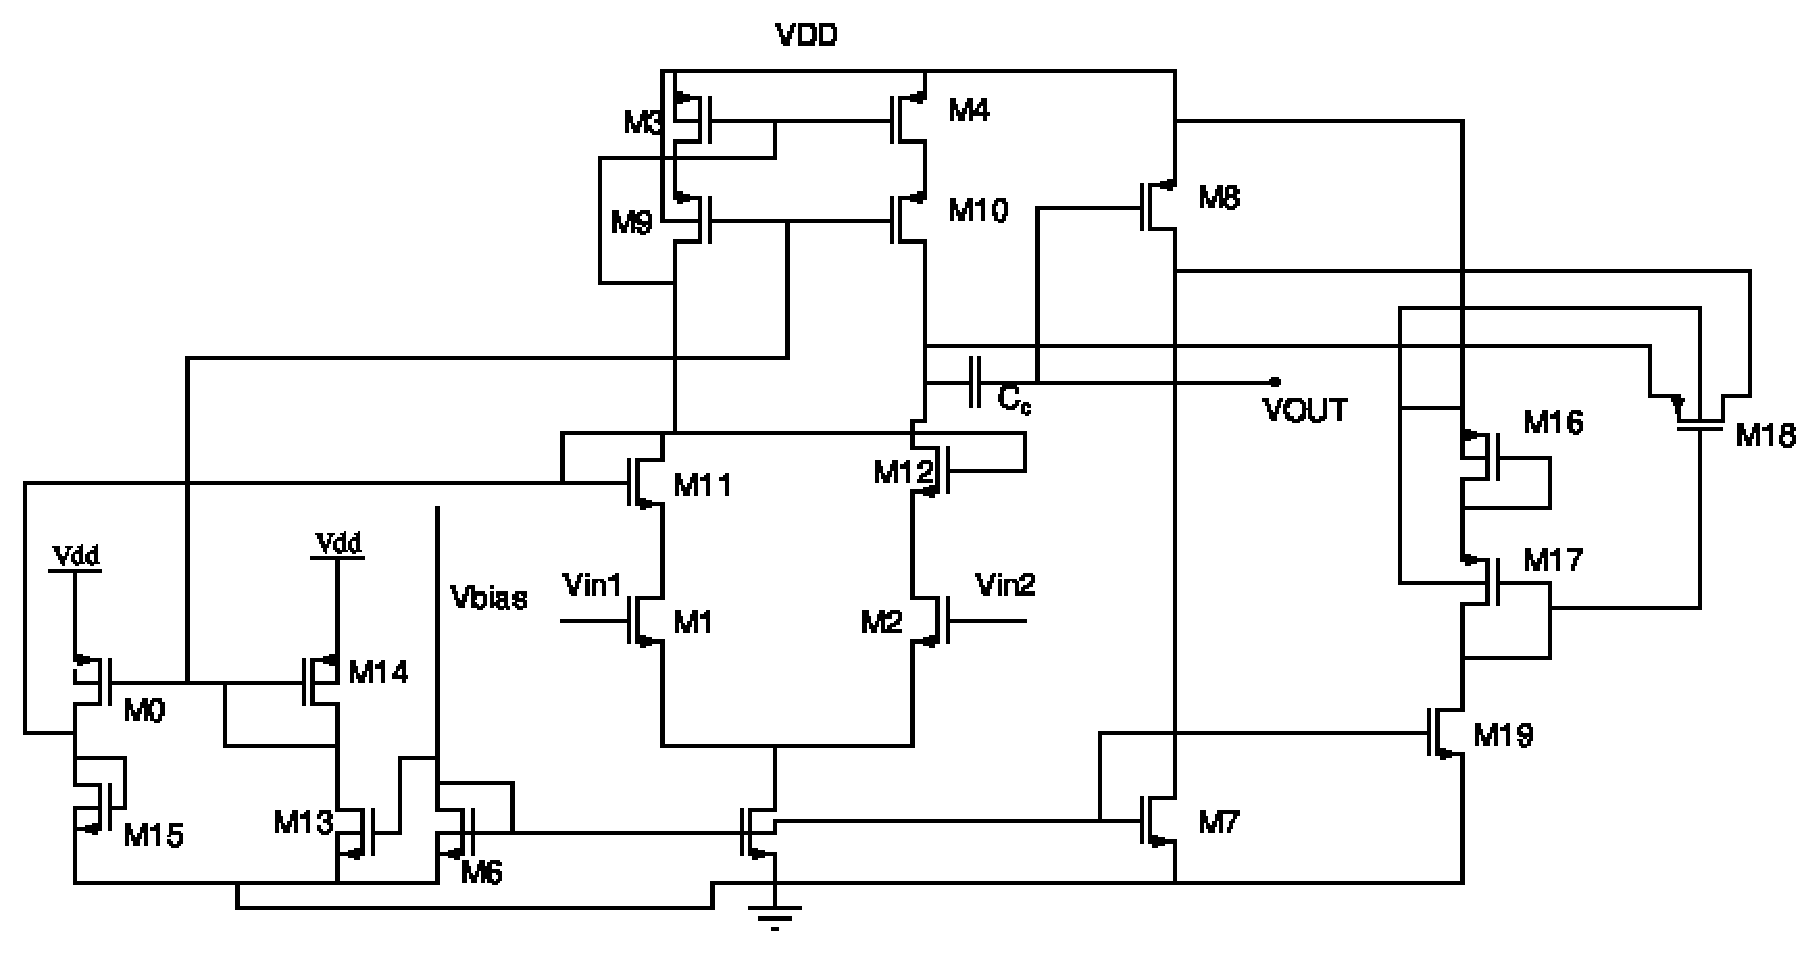
\includegraphics[width=0.85\textwidth]{circuit.eps}
    \caption{schematic of the two-stage telescopic operational amplifier.}
    \label{fig:ckt}
\end{figure*}

\noindent
\textbf{First Stage - Telescopic Differential Amplifier:}
The input stage comprises NMOS differential pair transistors M1 and M2, which receive the differential input signals IN\_N and IN\_P. The tail current source M5 provides bias current controlled by voltage $V_{BIAS}$. 

\noindent
The differential pair utilizes telescopic cascode configuration for high gain:
\begin{itemize}
    \item PMOS active loads M3 and M4 with cascode devices M9 and M10
    \item NMOS cascode transistors M11 and M12 stacked above M1 and M2
\end{itemize}

\noindent
This stacking of cascode transistors significantly increases the output impedance, thereby enhancing the overall voltage gain of the first stage.

\noindent
\textbf{Bias Voltages:}
\begin{itemize}
    \item $V_{B1}$: Biases the NMOS cascode transistors M11 and M12
    \item $V_{B2}$: Biases the PMOS cascode transistors M9 and M10
    \item $V_{BIAS}$: Controls the tail current source M5
\end{itemize}

\noindent
\textbf{Second Stage - Common-Source Amplifier:}
The second gain stage consists of NMOS common-source amplifier M7 with PMOS active load M8. This stage provides additional voltage gain and sufficient current drive capability for the load capacitance $C_L$ = 1 pF. 

\noindent
\textbf{Miller Compensation Network:}
The compensation capacitor $C_C$ = 452.907 fF connects the output to the input of the second stage, implementing Miller compensation. This ensures stability by creating a dominant pole and improving phase margin for closed-loop operation.

\noindent
\textbf{Bias Circuit:}
Figure~\ref{fig:bias_ckt} shows the bias circuit designed to generate the required bias voltage $V_{BIAS}$ = 650.575 mV. The circuit uses a current mirror configuration with transistors M20, M21, and M22, referenced to supply voltage $V_{DC}$ = 1.8 V. This bias circuit ensures stable biasing across process, voltage, and temperature variations.

\begin{figure}[H]
    \centering
    \includegraphics[width=0.3\textwidth]{bias_circuit.eps}
    \caption{Bias circuit generating $V_{BIAS}$ for the tail current source.}
    \label{fig:bias_ckt}
\end{figure}

\subsection{Transistor Sizing}
\noindent
The circuit was implemented with iterative optimization to meet the design specifications. Through multiple simulation iterations adjusting transistor widths, lengths, and bias voltages, the final optimized transistor dimensions were determined as listed in Table~\ref{tab:transistors}.

\begin{table}[H]
    \centering
    \caption{Final Transistor Dimensions}
    \label{tab:transistors}
    \begin{tabular}{@{}lcccc@{}}
        \toprule
        \textbf{Device} &  \textbf{W ($\mu$m)} & \textbf{L ($\mu$m)} & \textbf{M} \\
        \midrule
        M0 &  7.2 & 0.3 & 1 \\
        M1, M2 & 7 & 0.5 & 1 \\
        M3, M4 &  9 & 0.3 & 1 \\
        M5 (Tail NMOS) & 7.6 & 0.5 & 1 \\
        M6 & 1 & 0.5 & 1 \\
        M7 & 30 & 0.6 & 1 \\
        M8 & 72 & 0.5 & 1 \\
        M9, M10 & 5 & 0.3 & 1 \\
        M11, M12 & 7 & 0.5 & 1 \\
        M13 &  8 & 0.5 & 1 \\
        M14 &  2.4 & 0.3 & 1 \\
        M15 &  2.5 & 0.5 & 1 \\
        M16 &  1.26 & 0.3 & 1 \\
        M17 & 1 & 0.5 & 1 \\
        M18 &  11.725 & 0.3 & 1 \\
        M19 &  1.5 & 0.3 & 1 \\
        M20 &  1.32 & 0.18 & 1 \\
        M21 &  9 & 0.18 & 1 \\
        M22 &  4 & 0.18 & 1 \\
        \midrule
        $C_C$ & \multicolumn{3}{c}{452.907 fF} \\
        $C_L$ & \multicolumn{3}{c}{1 pF} \\
        \bottomrule
    \end{tabular}
\end{table}

\subsection{Operating Conditions}
\noindent
The amplifier operates under the following conditions:
\begin{itemize}
    \item Supply voltage: $V_{DD}$ = 1.8 V
    \item Input signal: Differential inputs IN\_P and IN\_N
    \item Input common-mode voltage: $V_{in}$ = 0.9 V (mid-rail)
    \item Load capacitance: $C_L$ = 1 pF
    \item Compensation capacitor: $C_C$ = 452.907 fF
    \item Bias voltage: $V_{BIAS}$ = 650.575 mV (generated from bias circuit)
\end{itemize}


% ================= SIMULATION RESULTS =================
\section{Simulation and Results}
\noindent
The designed telescopic operational amplifier was simulated using Cadence Virtuoso with the SCL 180 nm CMOS process design kit (PDK). This section presents the key simulation results including AC analysis, noise performance, PSRR, and CMRR.

\subsection{AC Analysis - Gain and Phase Response}
\noindent
Figure~\ref{fig:bode_mag} shows the gain magnitude and phase response of the amplifier. The DC gain achieved is 63 dB, significantly exceeding the target specification of 50 dB. The unity-gain bandwidth is measured at 100.78 MHz, closely matching the design target of 100 MHz. The gain-bandwidth product demonstrates the effectiveness of the Miller compensation strategy in achieving both high gain and adequate bandwidth.

\begin{figure}[H]
    \centering
    \includegraphics[width=0.48\textwidth]{ac_analysis.png}
    \caption{AC analysis showing gain magnitude (top) and phase response (bottom). DC gain = 63 dB, UGBW = 100.78 MHz, Phase Margin = 68\degree.}
    \label{fig:bode_mag}
\end{figure}

\noindent
The phase response, also shown in Fig.~\ref{fig:bode_mag}, indicates a phase margin of 68° at the unity-gain frequency. This is calculated as $180\degree + (-111\degree) = 69\degree$, which ensures stable operation with adequate damping in closed-loop configurations. A phase margin above 60° is generally considered sufficient for stable operation without significant overshoot or ringing in transient response.

\subsection{Noise Analysis}
\noindent
The input-referred noise spectral density is plotted in Fig.~\ref{fig:noise}. At mid-to-high frequencies where thermal noise dominates, the input-referred noise is approximately 15 nV/$\sqrt{\text{Hz}}$, which is excellent for this technology and transistor sizing. At low frequencies, flicker noise (1/f noise) becomes significant, reaching approximately 100 nV/$\sqrt{\text{Hz}}$ at 100 Hz, which is characteristic of CMOS devices. The low thermal noise floor indicates good transconductance in the input differential pair.

\begin{figure}[H]
    \centering
    \includegraphics[width=0.4\textwidth]{noise.png}
    \caption{Input-referred noise spectral density showing thermal noise floor at ~15 nV/$\sqrt{\text{Hz}}$ and 1/f noise at low frequencies.}
    \label{fig:noise}
\end{figure}

\subsection{Power Supply Rejection Ratio (PSRR)}
\noindent
The PSRR performance is shown in Fig.~\ref{fig:psrr}. The positive PSRR (PSRR+) measures the amplifier's ability to reject noise and variations on the positive supply rail. The achieved PSRR+ is 11.18 dB at low frequencies. While modest, this value is typical for single-stage telescopic architectures without dedicated supply rejection enhancement techniques. The PSRR degrades at higher frequencies as expected due to parasitic capacitances and reduced impedance paths.

\begin{figure}[H]
    \centering
    \includegraphics[width=0.4\textwidth]{psrr.png}
    \caption{Power Supply Rejection Ratio (PSRR+) showing 11.18 dB rejection at low frequencies.}
    \label{fig:psrr}
\end{figure}

\subsection{Common-Mode Rejection Ratio (CMRR)}
\noindent
The CMRR performance is illustrated in Fig.~\ref{fig:cmrr}. The amplifier achieves a CMRR of 58 dB at low frequencies, indicating good rejection of common-mode signals. This is primarily determined by the matching of the differential pair (M1, M2) and the output impedance of the tail current source (M5). The CMRR decreases at higher frequencies due to parasitic capacitance mismatches. A CMRR above 50 dB is generally considered adequate for most analog applications, making this design suitable for differential signal processing.

\begin{figure}[H]
    \centering
    \includegraphics[width=0.4\textwidth]{cmrr.png}
    \caption{Common-Mode Rejection Ratio (CMRR) showing 58 dB rejection at low frequencies.}
    \label{fig:cmrr}
\end{figure}

\subsection{Performance Summary}
\noindent
Table~\ref{tab:results} summarizes the achieved performance metrics compared to the target specifications. All primary design goals have been met or exceeded, demonstrating the effectiveness of the design approach.

\begin{table}[H]
    \centering
    \caption{Target vs. Achieved Performance Summary}
    \label{tab:results}
    \begin{tabular}{@{}lcc@{}}
        \toprule
        \textbf{Parameter} & \textbf{Target} & \textbf{Achieved} \\
        \midrule
        DC Gain (open-loop) & 50 dB & 63 dB \\
        Unity-Gain Bandwidth & 100 MHz & 100.78 MHz \\
        Phase Margin & $\geq$ 60\degree & 68\degree \\
        Input-referred Noise & Low & 15 nV/$\sqrt{\text{Hz}}$ \\
        PSRR+ & - & 11.18 dB \\
        CMRR & High & 58 dB \\
        Slew rate & High & 69 V/$\micro$s\\
        ICMR & - & 0.318V\\
        \bottomrule
    \end{tabular}
\end{table}

% ================= DISCUSSION =================
\section{Discussion}
\noindent
The implemented telescopic operational amplifier successfully meets all target specifications. The achieved DC gain of 63 dB exceeds the 50 dB requirement by 13 dB, demonstrating the effectiveness of the cascoded architecture in enhancing output impedance. The unity-gain bandwidth of 100.78 MHz closely matches the target, validating the compensation network design.

\noindent
The phase margin of 68° provides adequate stability margin for closed-loop operation with various feedback configurations. This suggests that the Miller compensation effectively addresses the two-pole system stability challenge inherent in two-stage amplifiers.

\noindent
The input-referred noise performance of 15 nV/$\sqrt{\text{Hz}}$ at high frequencies is excellent, significantly better than typical specifications for this technology. This low noise floor results from the proper sizing of the input differential pair (M1, M2) with adequate transconductance, achieved without excessive power consumption. The 1/f noise at low frequencies is typical for CMOS devices and can be further reduced if needed through increased device area or chopper stabilization techniques.

\noindent
The PSRR of 11.18 dB is modest but acceptable for many applications. The relatively low PSRR is inherent to the telescopic topology where supply variations directly affect the cascode devices. Applications requiring higher PSRR would benefit from regulated cascode techniques or additional supply filtering. The CMRR of 58 dB is good and demonstrates proper matching in the differential pair and adequate tail current source impedance.

\subsection{Key Design Tradeoffs}
\begin{itemize}
    \item \textit{Gain vs. Bandwidth:} The cascoded structure increases gain but adds poles at intermediate nodes. Careful sizing ensures these poles remain at sufficiently high frequencies to not affect stability.
    
    \item \textit{Noise vs. Power:} Larger input transistors reduce noise but increase power consumption and parasitic capacitances. The design achieves excellent noise performance (15 nV/$\sqrt{\text{Hz}}$) through optimal transconductance without excessive current.
    
    \item \textit{Output Swing vs. Gain:} The telescopic topology sacrifices output swing for gain due to transistor stacking. With a 1.8 V supply, adequate swing is maintained for most applications while achieving 63 dB gain.
    
    \item \textit{PSRR vs. Architecture:} The single-path current topology of telescopic amplifiers inherently limits PSRR. Better PSRR would require folded-cascode or regulated cascode techniques at the cost of higher power consumption.
\end{itemize}

\subsection{Potential Improvements}
\noindent
Future work could explore several enhancement strategies:
\begin{itemize}
    \item \textit{Improved PSRR:} Implementing regulated cascode or adding supply filtering circuits could significantly enhance power supply rejection.
    
    \item \textit{Dynamic Biasing:} Adaptive biasing techniques could improve power efficiency under varying load conditions.
    
    \item \textit{Layout Optimization:} Careful layout with parasitic extraction would verify post-layout performance and allow for matching optimization to further improve CMRR.
    
    \item \textit{Enhanced Output Swing:} Folded-cascode topology or rail-to-rail output stages could provide larger output voltage swing if required by the application.
\end{itemize}

% ================= CONCLUSION =================
\section{Conclusion}
\noindent
This work presented the complete design and analysis of a two-stage telescopic operational amplifier in 180 nm CMOS technology. Through systematic design methodology and iterative optimization, the implemented design achieved:
\begin{itemize}
    \item DC gain: 63 dB (target: $\geq$ 50 dB)
    \item Unity-gain bandwidth: 100.78 MHz (target: 100 MHz)
    \item Phase margin: 68° (target: $\geq$ 60°)
    \item Input-referred noise: 15 nV/$\sqrt{\text{Hz}}$ (excellent)
    \item CMRR: 58 dB (good)
    \item PSRR: 11.18 dB (acceptable)
\end{itemize}

\noindent
The telescopic architecture proved effective for applications requiring high gain and moderate bandwidth with reasonable power consumption at 1.8 V supply. The cascoded differential input stage combined with Miller compensation provides both high DC gain and stable frequency response. The excellent noise performance of 15 nV/$\sqrt{\text{Hz}}$ demonstrates the effectiveness of the transistor sizing strategy.

\noindent
The design successfully balances multiple performance metrics including gain, bandwidth, stability, and noise while maintaining moderate power consumption. The achieved CMRR of 58 dB ensures good differential operation, though the modest PSRR of 11.18 dB indicates that supply filtering may be beneficial in noise-sensitive applications.

\noindent
This design serves as a foundation for integration into larger mixed-signal systems such as switched-capacitor filters, pipelined ADCs, and precision instrumentation amplifiers. The systematic design approach and performance analysis presented here provide valuable insights into CMOS analog IC design tradeoffs and optimization strategies.

% ================= REFERENCES =================
\begin{thebibliography}{9}

\bibitem{razavi}
B. Razavi, \textit{Design of Analog CMOS Integrated Circuits}, 2nd ed. New York, NY: McGraw-Hill Education, 2016.

\bibitem{gray}
P. R. Gray, P. J. Hurst, S. H. Lewis, and R. G. Meyer, \textit{Analysis and Design of Analog Integrated Circuits}, 5th ed. Hoboken, NJ: John Wiley \& Sons, 2009.

\bibitem{johns}
D. A. Johns and K. Martin, \textit{Analog Integrated Circuit Design}, 2nd ed. Hoboken, NJ: John Wiley \& Sons, 2012.

\bibitem{baker}
R. J. Baker, \textit{CMOS: Circuit Design, Layout, and Simulation}, 3rd ed. Hoboken, NJ: John Wiley \& Sons, 2010.

\bibitem{sansen}
W. M. C. Sansen, \textit{Analog Design Essentials}. Dordrecht: Springer, 2006.

\bibitem{carusone}
T. C. Carusone, D. A. Johns, and K. W. Martin, \textit{Analog Integrated Circuit Design}, 2nd ed. Hoboken, NJ: John Wiley \& Sons, 2012.

\bibitem{telescopic_ref}
V. Soman, K. K. Gandhi, and M. Baskaran, "Analysis and design of a two stage telescopic OTA using SCL 180nm CMOS technology," in \textit{2023 International Conference on Networking and Communications (ICNWC)}, Chennai, India, 2023, pp. 1-6.

\bibitem{allen}
P. E. Allen and D. R. Holberg, \textit{CMOS Analog Circuit Design}, 2nd ed. New York: Oxford University Press, 2002.

\bibitem{laker}
K. R. Laker and W. M. C. Sansen, \textit{Design of Analog Integrated Circuits and Systems}. New York: McGraw-Hill, 1994.

\end{thebibliography}

\end{document}